% papel carta, lado unico, 11 puntos. tipo articulo
\documentclass[letter,oneside,11pt]{article}

% usar formato en español utf-8
\usepackage[spanish,es-nodecimaldot]{babel}
\usepackage[utf8]{inputenc}

% usar fuente helvetica
\usepackage{helvet}
\renewcommand{\familydefault}{\sfdefault}
\usepackage[T1]{fontenc}
\usepackage{textcomp}

% usar negrita en nombres de figura y cuadros
\usepackage[labelfont=bf]{caption}

% paquetes graficos
\usepackage{adjustbox}
\usepackage{graphicx}
\usepackage{pstricks}

% paquete de ecuaciones
\usepackage{amsmath}
% paquete para notacion exponencial
\usepackage{siunitx}

% personalizar los margenes de pagina
\usepackage{anysize}
\marginsize{3cm}{2cm}{2cm}{3cm}

% personalizacion de parrafo
\setlength{\parskip}{6pt}

% establecimiento del tamaño de pagina (necesario para incluir imagenes eps)
\special{papersize=215.9mm,279.4mm}

% personalizar encabezado y pie de pagina
\usepackage{fancyhdr}
\usepackage{lastpage}
\pagestyle{fancy}
\fancyhf{}
\fancyhead[LO]{Física Básica II}
\fancyhead[RO]{Momento de Inercia}
\fancyfoot[CO,CE]{\thepage\ de \pageref{LastPage}}

% paquete para indices, lista de figuras y cuadros
\usepackage[nottoc,notlof,notlot]{tocbibind}

% personalización del pdf
\usepackage[
    pdfauthor={Carlos Eduardo Caballero Burgoa},%
    pdftitle={Física Básica II},%
    pdfsubject={Momento de Inercia},%
    colorlinks,%
    citecolor=black,%
    filecolor=black,%
    linkcolor=black,%
    urlcolor=black,
    breaklinks]{hyperref}
\usepackage{breakurl}

% comando para generar una pagina en blanco
\newcommand{\blankpage}{
\newpage
\thispagestyle{empty}
\mbox{}
\newpage
}

\begin{document}

% caratula
\begin{titlepage}
    \begin{center}
        \begin{minipage}[]{.20\linewidth}
            \begin{flushleft}
                \includegraphics[width=2.6cm,height=2.6cm]{resources/umss.eps}
            \end{flushleft}
        \end{minipage}
        \begin{minipage}[]{.55\linewidth}
            \centering
            \large{\textbf{UNIVERSIDAD MAYOR DE SAN SIMÓN}} \newline
            \large{\textbf{FACULTAD DE CIENCIAS Y TECNOLOGÍA}} \newline
            \large{\textbf{CARRERA DE ELECTROMECÁNICA}} \newline
        \end{minipage}
        \begin{minipage}[]{.20\linewidth}
            \begin{flushright}
                \includegraphics[width=2.2cm,height=2.2cm]{resources/fcyt.eps}
            \end{flushright}
        \end{minipage}

        \vspace*{3.0cm}
        {\Large \textbf{FÍSICA BÁSICA II}}\\
        \vspace*{0.3cm}
        {\Large \textbf{Tarea de Investigación}}\\
        \vspace*{3.5cm}
        {\Large \textbf{MOMENTO DE INERCIA}}\\
    \end{center}

    \vspace*{6.5cm}
    \leftskip=7.95cm
    \noindent
    \textbf{Estudiante:}\\
    Caballero Burgoa, Carlos Eduardo.\\
    \newline
    \textbf{Docente:}\\
    Ing. Moreira Calizaya, René.\\
    \newline
    \textbf{Grupo:} J.\\
    \textbf{Fecha de entrega:} 1 de Mayo del 2021.\\
\end{titlepage}

% calcular el numero de paginas desde aqui
\clearpage
\setcounter{page}{1}

% generar indice
\tableofcontents
\newpage

\section{Introducción}
Cuando se analiza un movimiento traslacional y rectilíneo se considera a la masa
del objeto como una medida de su inercia. Por lo tanto, la masa es una medida de
la inercia de un cuerpo y es en este sentido, una medida de su resistencia al
cambio de velocidad.

Análogamente, al hacer que un objeto sólido rote o se mueva en trayectoria
curva, se observa una resistencia al cambio del movimiento rotacional. Esta
oposición del objeto al cambio de su rotación se conoce como inercia rotacional
o \textbf{momento de inercia}. En otras palabras, en el movimiento circular el
momento de inercia cumple el mismo rol que la masa juega en el movimiento
rectilíneo \cite{FISIC.CH}.

\section{Sistema discreto de partículas \cite{Sears}}
Se tiene un cuerpo formado por un sistema de partículas (véase la \textbf{Figura
\ref{figura1}}), con masas $m_1$, $m_2$, $m_3$, ..., $m_i$, ..., $m_{n-1}$,
$m_n$, a distancias perpendiculares $r_1$, $r_2$, $r_3$, ..., $r_i$, ...,
$r_{n-1}$, $r_n$ del eje de rotación.

\begin{figure}
\centering
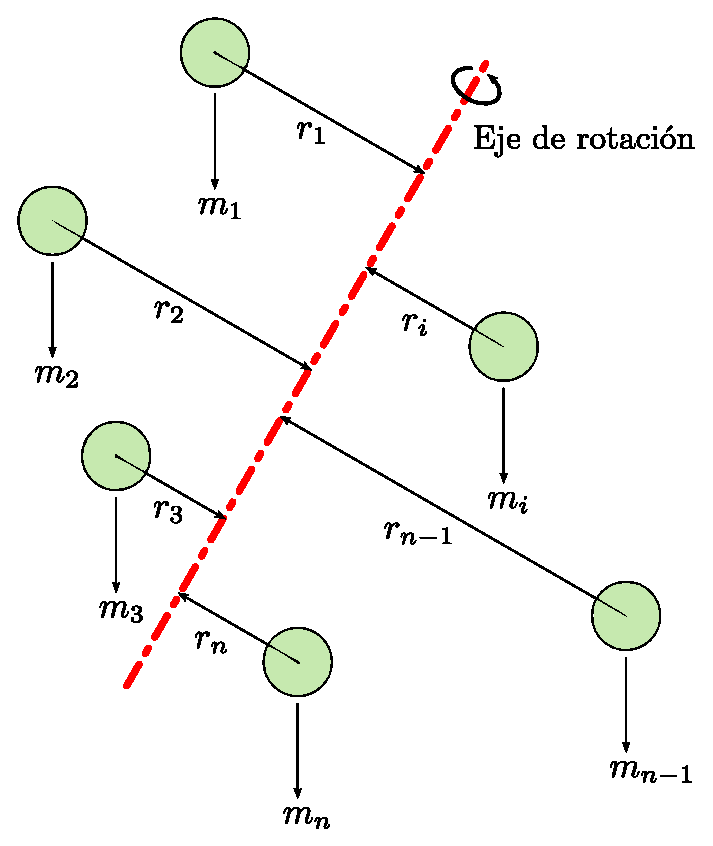
\includegraphics[width=0.42\textwidth]{resources/f1.eps}
\caption{Sistema de partículas girando alrededor de un eje.}
\label{figura1}
\end{figure}

Cuando este sistema de partículas gira alrededor de un eje fijo, la rapidez
$v_i$ de cada partícula esta dada por:

\begin{equation*}
    v = r \omega
\label{velocidad}
\end{equation*}

Donde $\omega$ es la magnitud de la velocidad angular del sistema de partículas
medida en $rad/s$. Cada partícula tiene un $r_i$ diferente, pero todas comparten
el mismo valor de $\omega$ (si es que consideramos el sistema de partículas como
un cuerpo rígido), por tanto la energía cinética de cada partícula es:

\begin{equation*}
    \frac{1}{2} m_i v^2_i = \frac{1}{2} m_i r^2_i \omega^2
\label{cinetica}
\end{equation*}

La energía cinética total del sistema de partículas es la suma de las energías
cinéticas de todas sus partículas:

\begin{equation*}
    K = \frac{1}{2} m_1 r^2_1 \omega^2 + ... + \frac{1}{2} m_n r^2_n \omega^2 = \sum_{i=1}^{n} \frac{1}{2} m_i r^2_i \omega^2
\label{cineticatotal1}
\end{equation*}

Sacando el factor común $\omega^2/2$ de la expresión, se obtiene:

\begin{equation*}
    K = \frac{1}{2} (m_1 r^2_1 + ... + m_n r^2_n ) \omega^2 = \frac{1}{2} \left( \sum_{i=1}^{n} m_i r^2_i \right) \omega^2
\label{cineticatotal2}
\end{equation*}

La cantidad entre paréntesis, que se obtiene multiplicando la masa de cada
partícula por el cuadrado de su distancia al eje de rotación y sumando los
productos, se denota con $I$, y es el \textbf{momento de inercia} del cuerpo
para este eje de rotación:

\begin{equation}
    I = m_1 r^2_1 + ... + m_n r^2_n = \sum_{i=1}^{n} m_i r^2_i
\label{momentodeinercia}
\end{equation}

Para un cuerpo con un eje de rotación dado y una masa total determinada, cuanto
mayor sea la distancia del eje a las partículas que constituyen el cuerpo, mayor
será el momento de inercia.

En términos del momento de inercia $I$, la \textbf{energía cinética de rotación}
$K$ de un cuerpo rígido es:

\begin{equation}
    K = \frac{1}{2} I \omega^2
\label{cineticarotacional}
\end{equation}

Entonces, cuanto mayor sea el momento de inercia, mayor será la energía cinética
de un cuerpo rígido que gira con una rapidez angular $\omega$. Y sabiendo que la
energía cinética de un cuerpo es igual al trabajo efectuado para acelerar ese
cuerpo desde el reposo, podemos asumir que cuanto mayor sea el momento de
inercia de un cuerpo, más difícil sera ponerlo a girar si está en reposo, y más
difícil será detener su rotación si ya está girando.

\begin{minipage}[b]{.4\linewidth}
\textbf{Ejemplo 1}:\\
Se tiene un sistema de 6 partículas como se muestra en la figura. \\

a) Calcular el momento de inercia del sistema para el eje de rotación $y = 6$, \\
b) Calcular la energía cinética rotacional si el sistema gira con una rapidez
angular $\omega = 4.0 [rad/s]$.
\end{minipage}\hfill
\begin{minipage}{.5\linewidth}
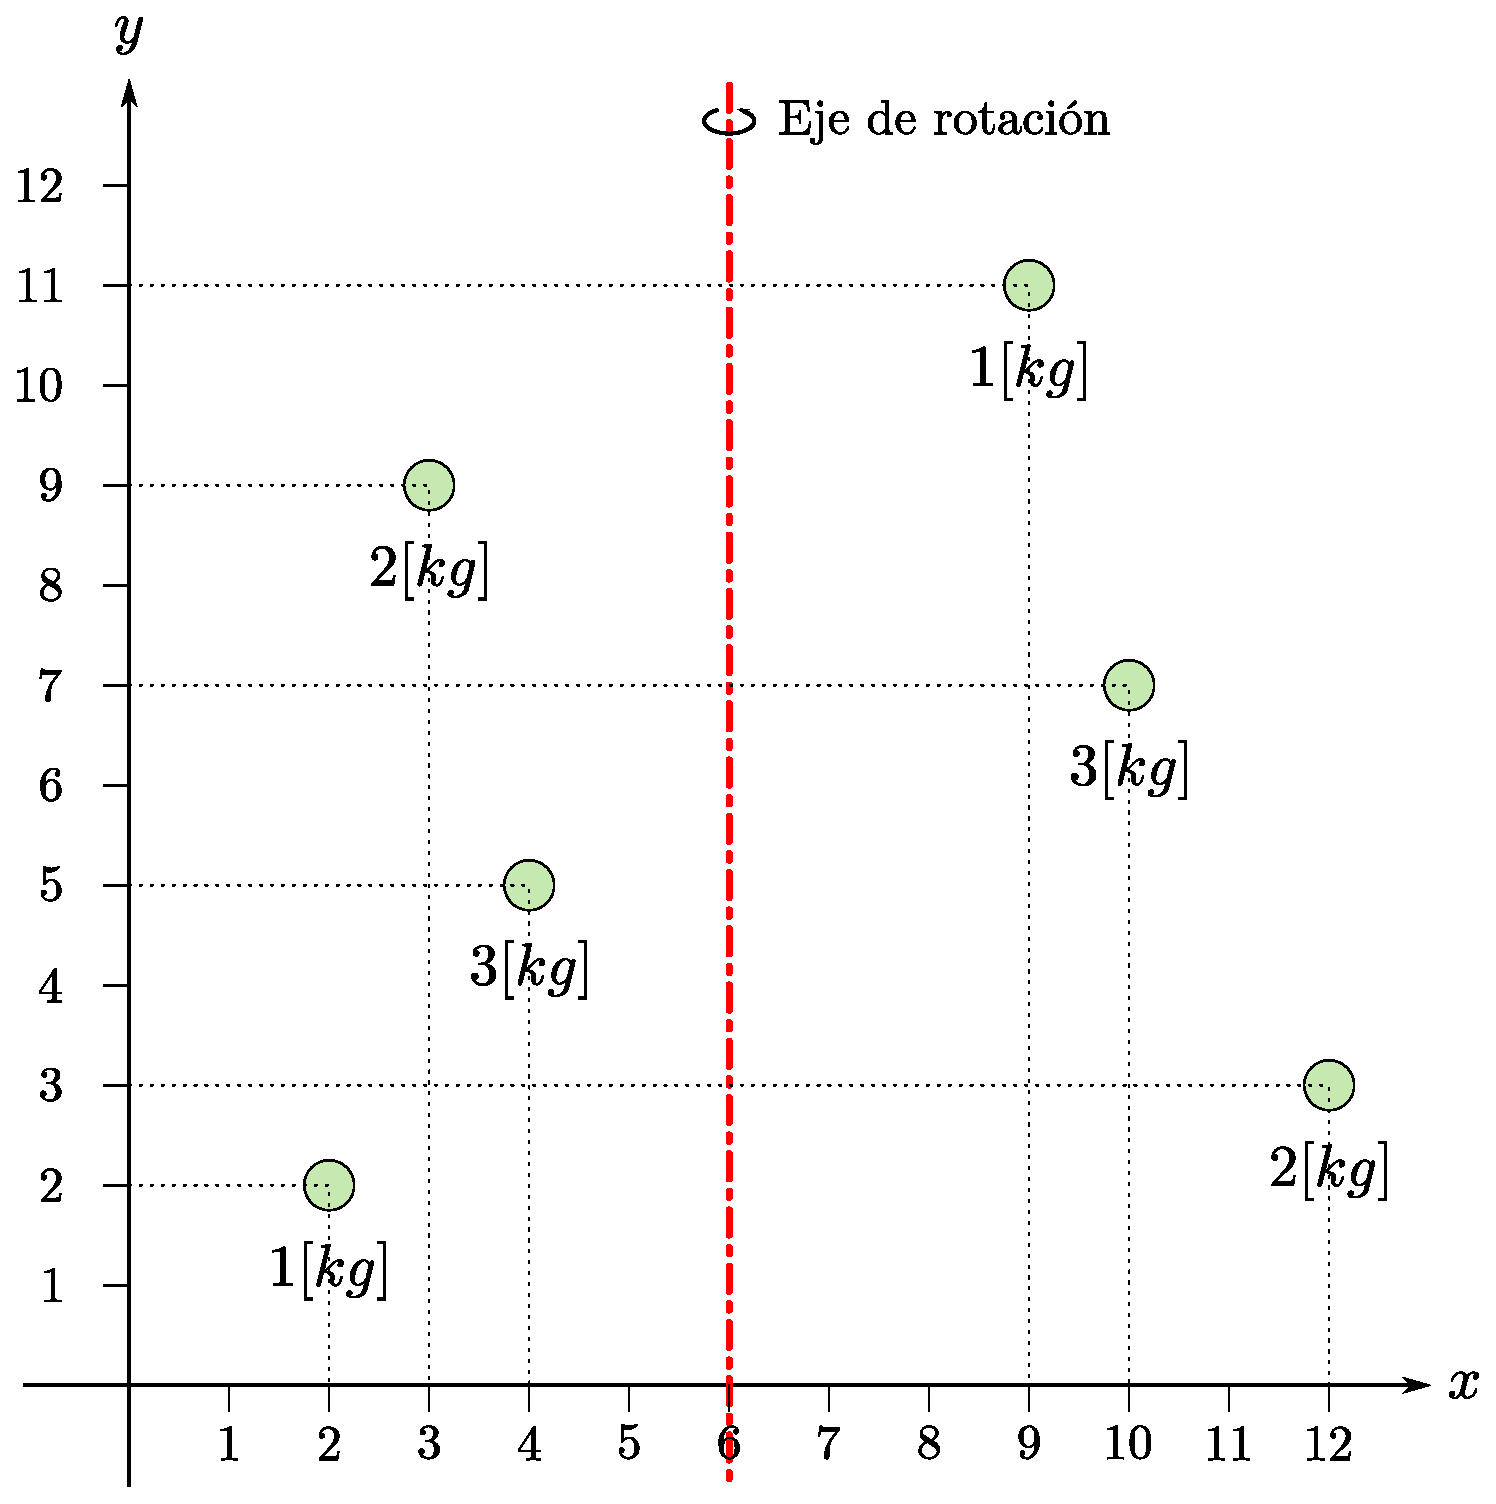
\includegraphics[width=0.95\textwidth]{resources/f2.eps}
\end{minipage}

\begin{minipage}[b]{.9\linewidth}
\textbf{Solución}:\\
a) Para calcular el momento de inercia se utilizara la \textbf{ecuación
(\ref{momentodeinercia})}, y se calculará la distancia perpendicular
aprovechando que el eje es vertical.

\begin{equation*}
    I = \sum_{i=1}^{6} m_i r^2_i = 1 (4)^2 + 2(3)^2 + 3(2)^2 + 1(3)^2 + 3(4)^2 + 2(6)^2 = 175 [kg\, m^2]
\end{equation*}

b) Una vez calculado el momento de inercia para el eje propuesto, se puede
calcular la energía cinética con la \textbf{ecuación
(\ref{cineticarotacional})}:

\begin{equation*}
    K = \frac{1}{2} I \omega^2 =  \frac{1}{2} \left(175 [kg\, m^2]\right) \left(4.0 \left[\frac{rad}{s^2}\right]\right) = 350 [J]
\end{equation*}
\end{minipage}
\\

\begin{minipage}[b]{.4\linewidth}
\textbf{Ejemplo 2}:\\
Se tiene el sistema de 6 partículas anteriormente citado como se muestra en la
figura. \\

a) Calcular el momento de inercia del sistema para el eje de rotación $y = x$, \\
b) Calcular la energía cinética rotacional si el sistema gira con una rapidez
angular $\omega = 4.0 [rad/s]$.
\end{minipage}\hfill
\begin{minipage}{.5\linewidth}
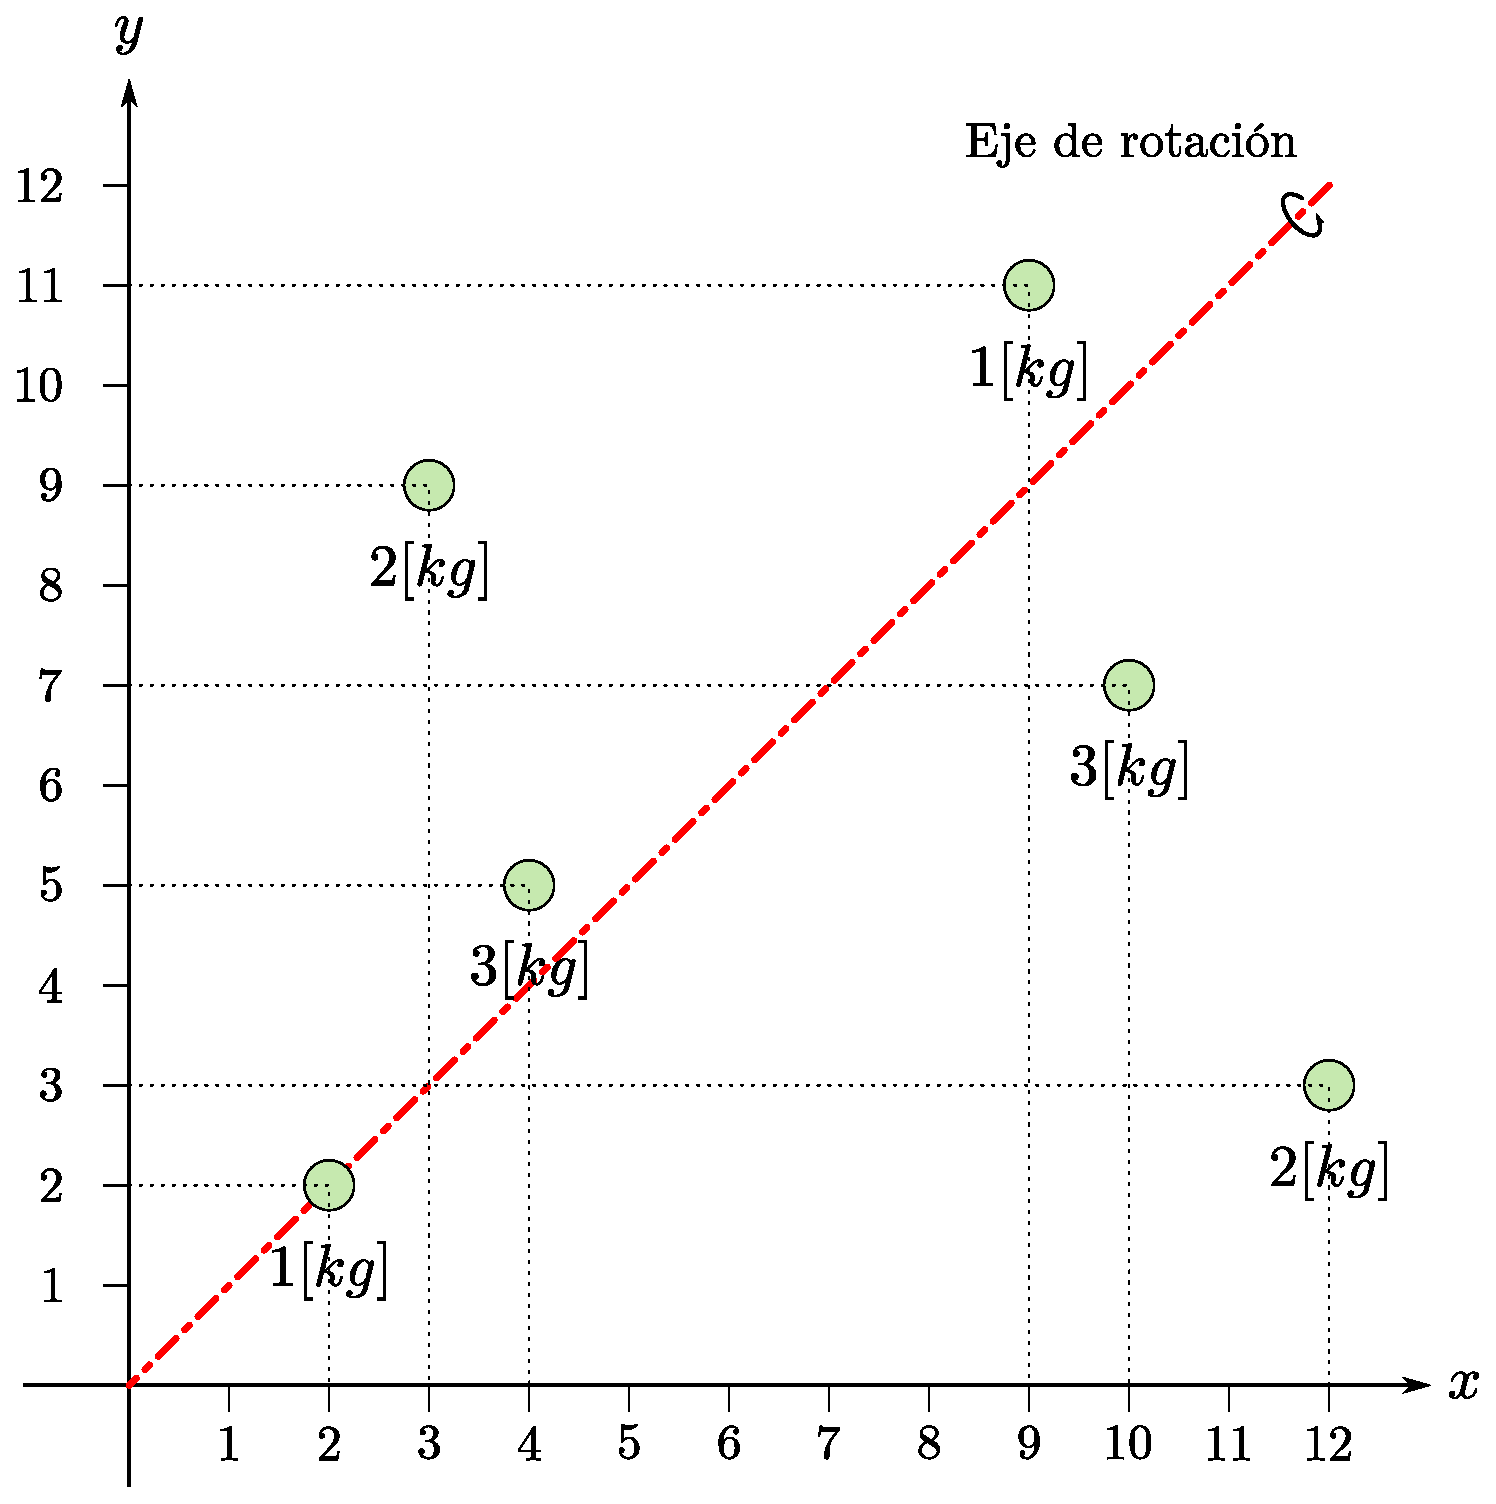
\includegraphics[width=0.95\textwidth]{resources/f3.eps}
\end{minipage}

\begin{minipage}[b]{.9\linewidth}
\textbf{Solución}:\\
a) Para calcular el momento de inercia se utilizará la \textbf{ecuación
(\ref{momentodeinercia})}, y considerando que el eje es diagonal al sistema de
referencia, se debe calcular la distancia perpendicular a tal eje: \\

Ecuación de la recta:
\begin{equation*}
    x - y = 0
\end{equation*}

Distancia de una recta a un punto:
\begin{equation*}
    d = \frac{| A x + B y + C |}{\sqrt{A^2 + B^2}}
\end{equation*}

Por tanto: \\
\begin{equation*}
    d_1(2,2) = \frac{| 1 (2) - 1 (2) |}{\sqrt{1^2 + (-1)^2}} = \frac{|2 - 2|}{\sqrt{2}} = 0
\end{equation*}
\begin{equation*}
    d_2(3,9) = \frac{| 1 (3) - 1 (9) |}{\sqrt{1^2 + (-1)^2}} = \frac{|3 - 9|}{\sqrt{2}} = \frac{6}{\sqrt{2}}
\end{equation*}
\end{minipage}

\begin{minipage}[b]{.9\linewidth}
\begin{equation*}
    d_3(4,2) = \frac{| 1 (4) - 1 (2) |}{\sqrt{1^2 + (-1)^2}} = \frac{|4 - 2|}{\sqrt{2}} = \frac{2}{\sqrt{2}}
\end{equation*}
\begin{equation*}
    d_4(9,11) = \frac{| 1 (9) - 1 (11) |}{\sqrt{1^2 + (-1)^2}} = \frac{|9 - 11|}{\sqrt{2}} = \frac{2}{\sqrt{2}}
\end{equation*}
\begin{equation*}
    d_5(10,7) = \frac{| 1 (10) - 1 (7) |}{\sqrt{1^2 + (-1)^2}} = \frac{|10 - 7|}{\sqrt{2}} = \frac{3}{\sqrt{2}}
\end{equation*}
\begin{equation*}
    d_6(12,3) = \frac{| 1 (12) - 1 (3) |}{\sqrt{1^2 + (-1)^2}} = \frac{|12 - 3|}{\sqrt{2}} = \frac{9}{\sqrt{2}}
\end{equation*}
\\

Con las distancias determinadas, se calcula el momento de inercia:
\begin{equation*}
    I = \sum_{i=1}^{6} m_i r^2_i = 1 (0) + 2\left(\frac{6}{\sqrt{2}}\right)^2 + 3\left(\frac{2}{\sqrt{2}}\right)^2 + 1\left(\frac{2}{\sqrt{2}}\right)^2 + 3\left(\frac{3}{\sqrt{2}}\right)^2 + 2\left(\frac{9}{\sqrt{2}}\right)^2
\end{equation*}
\begin{equation*}
    I = 2 \left(\frac{36}{2}\right) + 3 \left(\frac{4}{2}\right) + 1 \left(\frac{4}{2}\right) + 3 \left(\frac{9}{2}\right) + 2 \left(\frac{81}{2}\right) = \frac{277}{2} [kg\, m^2]
\end{equation*}
\\

b) Una vez calculado el momento de inercia para el eje propuesto, se puede
calcular la energía cinética con la \textbf{ecuación
(\ref{cineticarotacional})}:

\begin{equation*}
    K = \frac{1}{2} I \omega^2 =  \frac{1}{2} \left(\frac{277}{2} [kg\, m^2]\right) \left(4.0 \left[\frac{rad}{s^2}\right]\right) = 277 [J]
\end{equation*}
\end{minipage}

\begin{minipage}[c]{.4\linewidth}
\textbf{Ejemplo 3}:\\
Se tiene el sistema de 4 partículas como se muestra en la figura cuyas masas y
posiciones son:

\begin{equation*}
    m_1 = 1 [kg]\; p_1 = (2,5,3)
\end{equation*}
\begin{equation*}
    m_2 = 2 [kg]\; p_2 = (6,0,0)
\end{equation*}
\begin{equation*}
    m_3 = 3 [kg]\; p_3 = (6,8,1)
\end{equation*}
\begin{equation*}
    m_4 = 4 [kg]\; p_4 = (12,2,1)
\end{equation*}

a) Calcular el momento de inercia del sistema para el eje de rotación que pasa
por los puntos $A = (0,2,1)$ y $B = (12,11,5)$. \\
b) Calcular la energía cinética rotacional si el sistema gira con una rapidez
angular $\omega = 4.0 [rad/s]$.
\end{minipage}\hfill
\begin{minipage}{.5\linewidth}
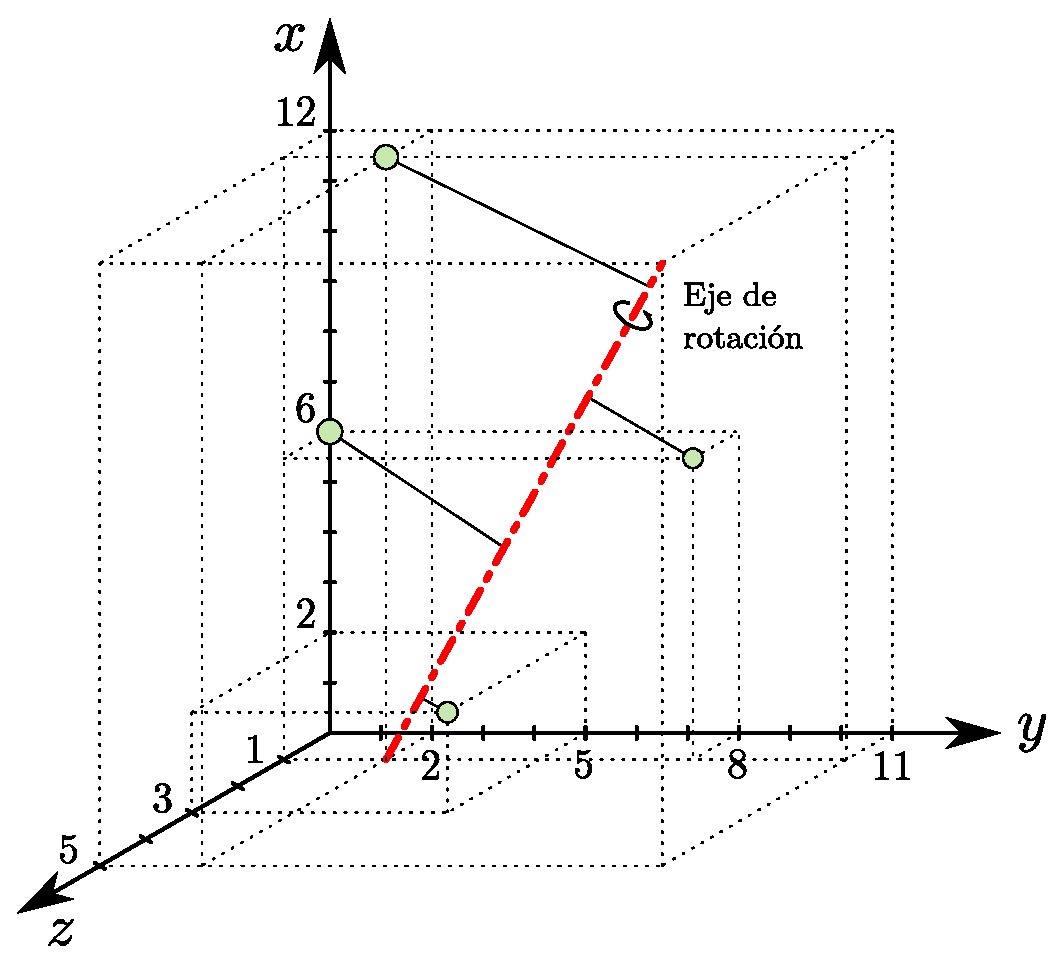
\includegraphics[width=0.95\textwidth]{resources/f4.eps}
\end{minipage}
\\
\\

\begin{minipage}[b]{.9\linewidth}
\textbf{Solución}:\\
a) Para calcular el momento de inercia se utilizará la \textbf{ecuación
(\ref{momentodeinercia})}, y se usaran operaciones vectoriales para facilitar el
trabajo con tres dimensiones: \\

Vector posición del eje:
\begin{equation*}
    \vec{r}_{AB} = B - A = (12,11,5) - (0,2,1) = (12,9,4)
\end{equation*}

Distancia mínima de un punto $P_i$ a la linea de $A$ a $B$:
\begin{equation*}
    d = | \vec{r}_{AP_i} | \left(\frac{| \vec{r}_{AP_i} \times \vec{r}_{AB} |}{|\vec{r}_{AP_i}| |\vec{r}_{AB}|} \right)
\end{equation*}

Por tanto: \\
\begin{equation*}
    d_1(2,5,3) = |(2,3,2)| \left(\frac{|(2,3,2)\times(12,9,4)|}{|(2,3,2)||(12,9,4)|}\right) = 1.5988
\end{equation*}
\begin{equation*}
    d_2(6,0,0) = |(6,-2,-1)| \left(\frac{|(6,-2,-1)\times(12,9,4)|}{|(6,-2,-1)||(12,9,4)|}\right) = 5.5341
\end{equation*}
\begin{equation*} 
    d_3(6,8,1) = |(6,6,0)| \left(\frac{|(6,6,0)\times(12,9,4)|}{|(6,6,0)||(12,9,4)|}\right) = 2.4748
\end{equation*}
\begin{equation*}
    d_4(12,2,1) = |(12,0,0)| \left(\frac{|(12,0,0)\times(12,9,4)|}{|(12,0,0)||(12,9,4)|}\right) = 7.6130
\end{equation*}
\\

Con las distancias determinadas, se calcula el momento de inercia:
\end{minipage}

\begin{minipage}[b]{.9\linewidth}
\begin{equation*}
    I = \sum_{i=1}^{4} m_i r^2_i = 1 (1.5988)^2 + 2 (5.5341)^2 + 3 (2.4748)^2 + 4 (7.6130)^2 = 314.02 [kg\, m^2]
\end{equation*}

b) Una vez calculado el momento de inercia para el eje propuesto, se puede
calcular la energía cinética con la \textbf{ecuación
(\ref{cineticarotacional})}:

\begin{equation*}
    K = \frac{1}{2} I \omega^2 =  \frac{1}{2} (314.02 [kg\, m^2]) \left(4.0 \left[\frac{rad}{s^2}\right]\right) = 628.03 [J]
\end{equation*}
\end{minipage}

\section{Teorema de los ejes paralelos \cite{Sears}}

Considérese dos ejes de rotación paralelos en un sistema discreto de partículas
(véase la \textbf{Figura \ref{figura5}}), uno de estos ejes ubicado en el centro
de masa $O = (0,0)$ y otro en un punto $P = (a,b)$.

\begin{figure}
\centering
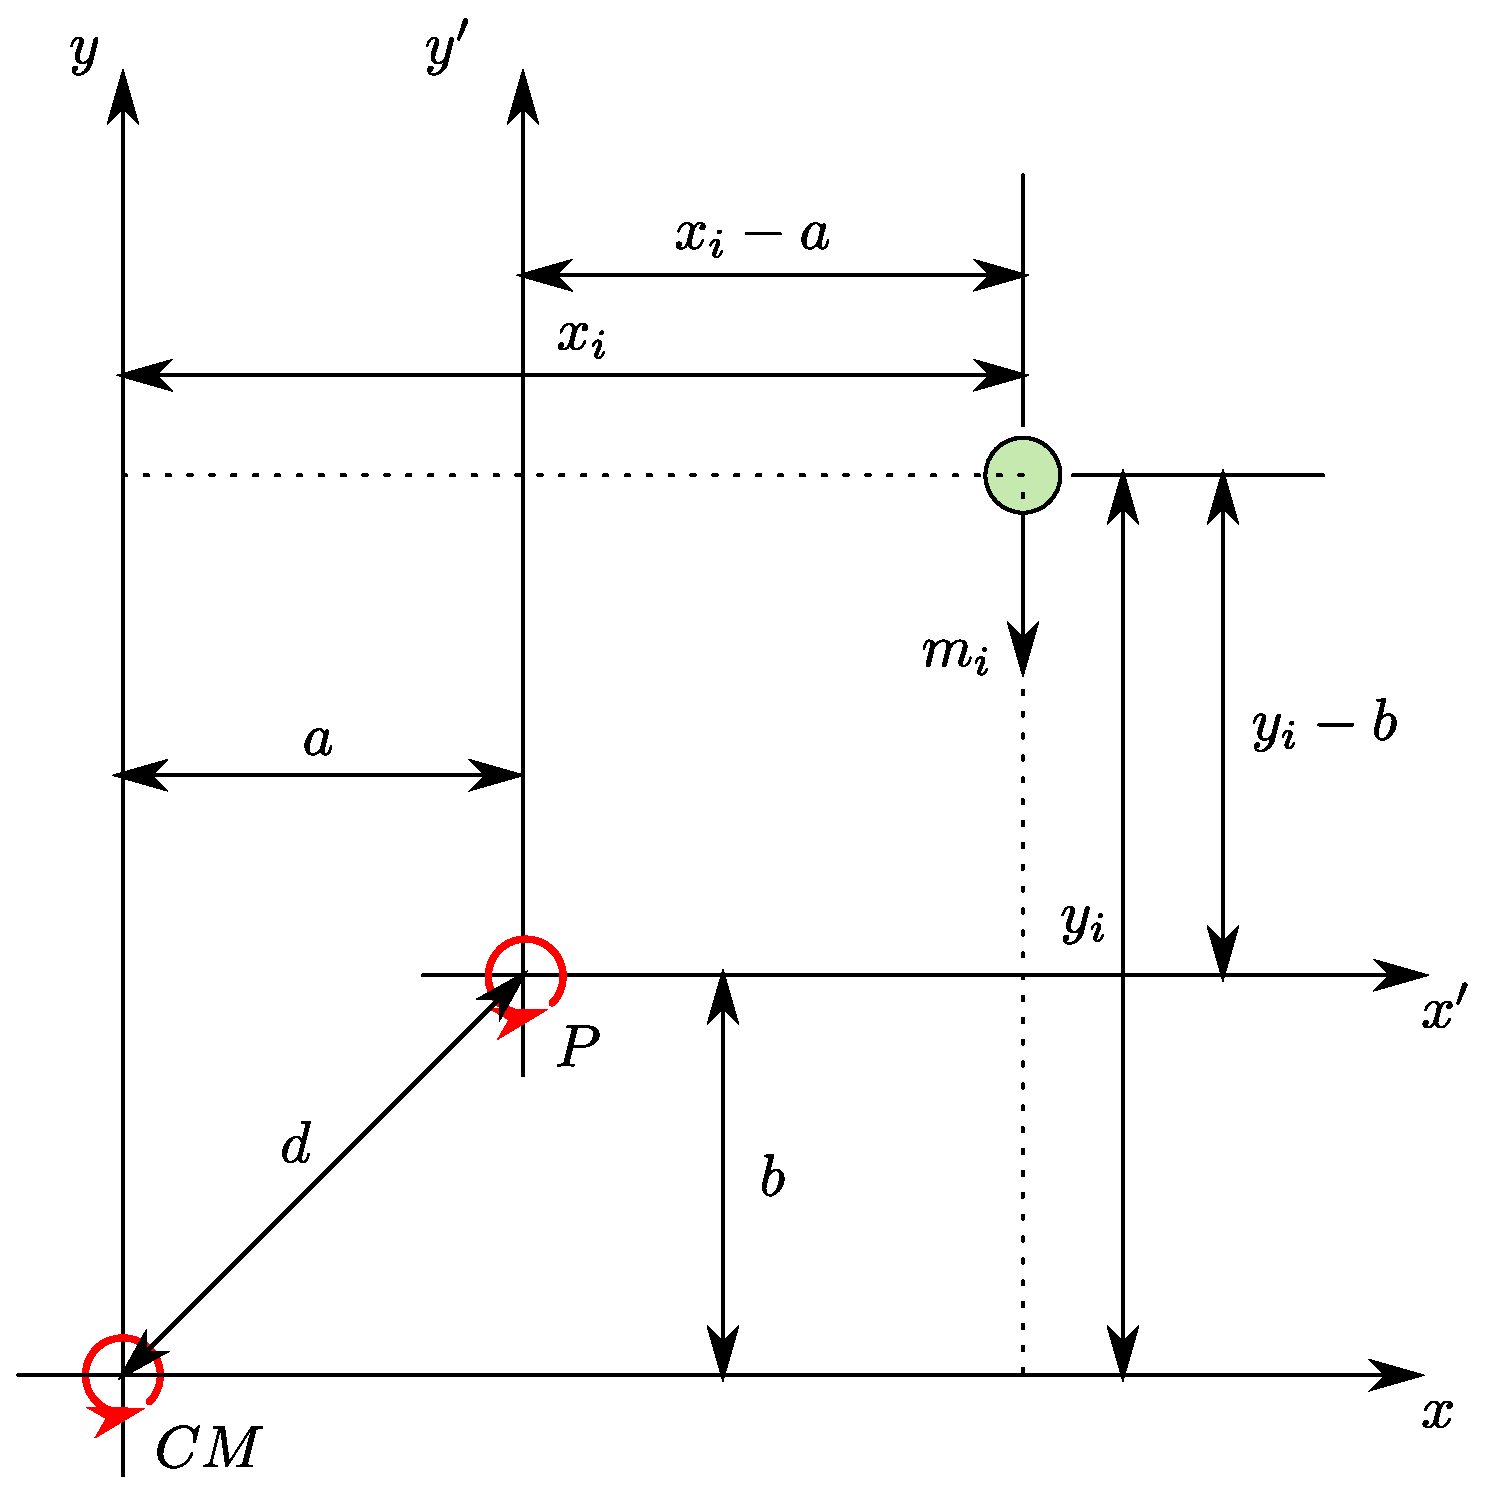
\includegraphics[width=0.50\textwidth]{resources/f5.eps}
\caption{Dos ejes paralelos y su relación con una partícula de un sistema discreto.}
\label{figura5}
\end{figure}

El momento de inercia para el centro de masa es:

\begin{equation*}
    I_{CM} = \sum_{i=1}^{n} m_i\, (x^2_i + y^2_i)
\end{equation*}

Mientras que el momento de inercia  para el punto $P$ es:

\begin{equation*}
    I_{P} = \sum_{i=1}^{n} m_i\, [ (x_i-a)^2 + (y_i-b)^2 ]
\end{equation*}

Expandiendo los cuadrados y reagrupando los términos, se obtiene:

\begin{equation*}
    I_{P} = \sum_{i=1}^{n} m_i\, (x^2_i + y^2_i) - 2a \sum_{i=1}^{n} m_i\, x_i - 2b \sum_{i=1}^{n} m_i\, y_i + (a^2 + b^2) \sum_{i=1}^{n} m_i
\end{equation*}

Considerando que el centro de masa del sistema se encuentra en el origen
$(0,0)$, sabemos que:

\begin{equation*}
    \sum_{i=1}^{n} m_i\, x_i = 0
\end{equation*}
\begin{equation*}
    \sum_{i=1}^{n} m_i\, y_i = 0
\end{equation*}

Por tanto el momento de inercia $I_P$, resulta:

\begin{equation*}
    I_{P} = \sum_{i=1}^{n} m_i\, (x^2_i + y^2_i) + (a^2 + b^2) \sum_{i=1}^{n} m_i
\end{equation*}
\begin{equation*}
    I_{P} = I_{CM} + (a^2 + b^2) \sum_{i=1}^{n} m_i
\end{equation*}
\begin{equation*}
    I_{P} = I_{CM} + (a^2 + b^2) M
\end{equation*}

Considerando la relación pitagórica entre las variables $a$, $b$, y $d$:

\begin{equation*}
    d^2 = a^2 + b^2
\end{equation*}

Por tanto:

\begin{equation}
    I_{P} = I_{CM} + M\, d^2
\label{steiner}
\end{equation}

Este es el teorema de los ejes paralelos, también conocido como teorema de 
\emph{Huygens–Steiner}, o simplemente como teorema de \emph{Steiner}, puede
utilizarse para determinar el momento de inercia o segundo momento de área de
un cuerpo rígido respecto a cualquier eje, a partir del momento de inercia del
cuerpo respecto a un eje paralelo al anterior que pase a través del centro de
masas del objeto, de la masa del objeto y de la distancia medida
perpendicularmente entre ambos ejes \cite{WIKI1}.

\section{Sistema continuo de partículas \cite{Sears}}

Para el calculo de momentos de inercia en distribuciones continuas de masa, se
transforma la masa $m_i$ a un diferencial de masa $dm$ y la sumatoria de las
partículas a una integral, la \textbf{Ecuación \ref{momentodeinercia}} se
transforma en:

\begin{equation}
    I = \int_{M} r^2\, dm
\label{solidorigido}
\end{equation}

Para la resolución de esta integral, se debe representar $r$ y $dm$ en términos
de la variable de integración. Para eso puede usarse el concepto de densidad:

\begin{equation}
    \rho = \frac{dm}{dv}
\label{densidad}
\end{equation}

Por tanto:

\begin{equation*}
    dm = \rho\, dv
\end{equation*}

Y reemplazando en la \textbf{Ecuación \ref{solidorigido}}, obtenemos:

\begin{equation*}
    I = \int_{V} r^2\, \rho\, dv
\end{equation*}

Si es que la densidad del objeto es uniforme, $rho$ puede salir de la integral:

\begin{equation}
    I = \rho \int_{V} r^2\, dv
\end{equation}

Dependiendo del tipo de objeto pueden usarse tres diferentes tipos de densidad,
en el cambio de variable de la integral.

Por ejemplo en coordenadas cartesianas se tienen:

\begin{itemize}
\item Densidad lineal de masa:
\begin{equation*}
    dm = \lambda\, dx
\end{equation*}

\item Densidad superficial de masa:
\begin{equation*}
    dm = \sigma\, dx\, dy
\end{equation*}

\item Densidad volumétrica de masa:
\begin{equation*}
    dm = \rho\, dx\, dy\, dz
\end{equation*}
\end{itemize}

\section{Calculo de momentos de inercia}

\subsection{Varilla delgada horizontal}
El procedimiento para hallar el momento de inercia de una varilla delgada (véase
la \textbf{Figura \ref{figura6}}) con eje en el centro de masa y perpendicular a
su longitud ($L$), es el siguiente:

\begin{figure}
\centering
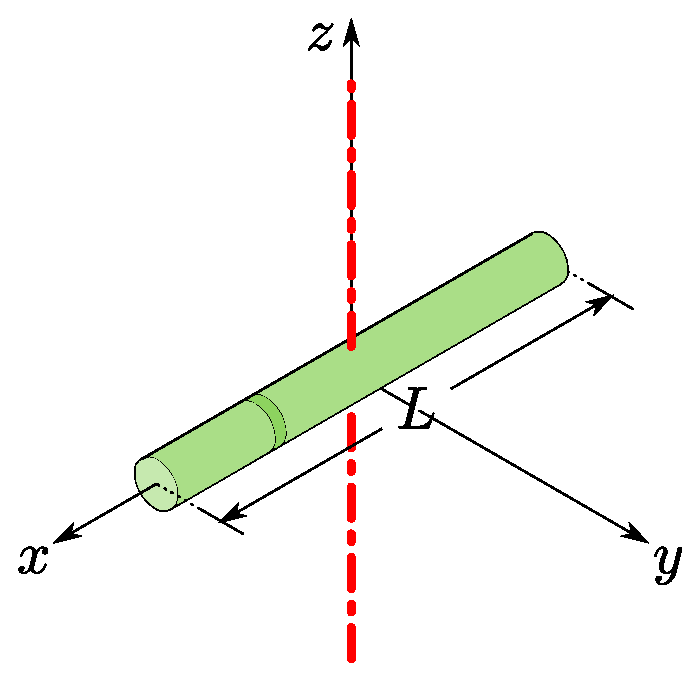
\includegraphics[scale=0.5]{resources/f6.eps}
\caption{Varilla delgada horizontal.}
\label{figura6}
\end{figure}

Considerando la \textbf{Ecuación (\ref{solidorigido})}:

\begin{equation*}
    I = \int_{M} r^2\, dm
\tag{4}
\end{equation*}

Asumiendo la distribución homogénea y longitudinal de la masa:

\begin{equation*}
    \lambda = \frac{dm}{dl}
\end{equation*}

Por tanto:

\begin{equation}
    dm = \lambda\, dl
\label{dm1}
\end{equation}

Para cada diferencial, se sabe que $r$ es equivalente al valor de
$|l|$:

\begin{equation}
    r^2 = l^2
\label{r1}
\end{equation}

Reemplazando (\ref{r1}) y (\ref{dm1}) en (\ref{solidorigido}):

\begin{equation*}
    I = \int_{M} r^2\, dm = \int_{-L/2}^{L/2} l^2\, \lambda\, dl = \lambda \int_{-L/2}^{L/2} l^2\, dl = \lambda\, \frac{l^3}{3} \Biggr|_{-L/2}^{L/2} = \lambda \left( \frac{(\frac{L}{2})^3}{3} - \frac{(-\frac{L}{2})^3}{3} \right)
\end{equation*}
\begin{equation}
    I = \lambda\, \frac{L^3}{12}
\label{resultado1}
\end{equation}

A partir de la ecuación (\ref{dm1}) sabemos que:

\begin{equation*}
    M = \lambda\, L
\end{equation*}

Despejando $\lambda$ y reemplazando en la ecuación (\ref{resultado1}):

\begin{equation*}
    I = \frac{1}{12} \left( \frac{M}{L} \right) L^3
\end{equation*}

Resultando finalmente:

\begin{equation}
    I = \frac{1}{12}\, M\, L^2
\end{equation}

\subsection{Anillo delgado horizontal}
El procedimiento para hallar el momento de inercia de un anillo delgado (véase
la \textbf{Figura \ref{figura7}}) con eje en el centro de masa y perpendicular a
su radio ($R$), es el siguiente:

\begin{figure}
\centering
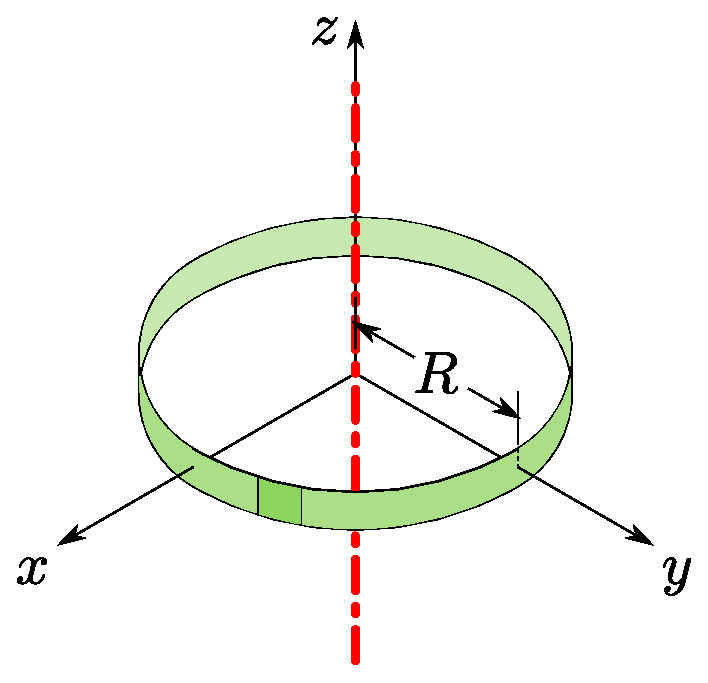
\includegraphics[scale=0.5]{resources/f7.eps}
\caption{Anillo delgado horizontal.}
\label{figura7}
\end{figure}

Considerando la \textbf{Ecuación (\ref{solidorigido})}:

\begin{equation*}
    I = \int_{M} r^2\, dm
\tag{4}
\end{equation*}

Asumiendo la distribución homogénea y longitudinal de la masa, y usando un
sistema de referencia polar:

\begin{equation*}
    \lambda = \frac{dm}{dl} = \frac{dm}{R\, d\theta}
\end{equation*}

Por tanto:

\begin{equation}
    dm = \lambda\, R\, d\theta
\label{dm2}
\end{equation}

Para cada diferencial, se sabe que $r$ es equivalente al valor de
$R$:

\begin{equation}
    r = R
\label{r2}
\end{equation}

Reemplazando (\ref{r2}) y (\ref{dm2}) en (\ref{solidorigido}):

\begin{equation*}
    I = \int_{M} r^2\, dm = \int_{0}^{2\pi} R^2\, \lambda\, R\, d\theta = \lambda\, R^3\, \int_{0}^{2\pi} d\theta = \lambda\, R^3\, (\theta \Biggr|_{0}^{2\pi})
\end{equation*}
\begin{equation}
    I = \lambda\, R^3\, 2\pi
\label{resultado2}
\end{equation}

A partir de la ecuación (\ref{dm2}) sabemos que:

\begin{equation*}
    M = \lambda\, R\, 2\pi
\end{equation*}

Despejando $\lambda$ y reemplazando en la ecuación (\ref{resultado2}):

\begin{equation*}
    I = \left( \frac{M}{2\pi\, R} \right) R^3\, 2\pi
\end{equation*}

Resultando finalmente:

\begin{equation}
    I = M\, R^2
\end{equation}

\subsection{Anillo delgado vertical}
El procedimiento para hallar el momento de inercia de un anillo delgado (véase
la \textbf{Figura \ref{figura8}}) con eje en el centro de masa y paralelo a
su radio ($R$), es el siguiente:

\begin{figure}
\centering
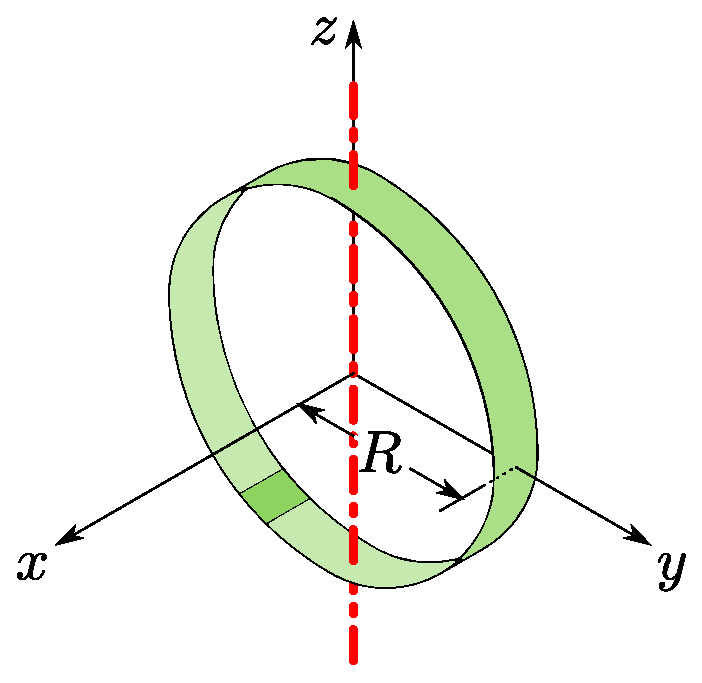
\includegraphics[scale=0.5]{resources/f8.eps}
\caption{Anillo delgado vertical.}
\label{figura8}
\end{figure}

Considerando la \textbf{Ecuación (\ref{solidorigido})}:

\begin{equation*}
    I = \int_{M} r^2\, dm
\tag{4}
\end{equation*}

Asumiendo la distribución homogénea y longitudinal de la masa, y usando un
sistema de referencia polar:

\begin{equation*}
    \lambda = \frac{dm}{dl} = \frac{dm}{R\, d\theta}
\end{equation*}

Por tanto:

\begin{equation}
    dm = \lambda\, R\, d\theta
\label{dm3}
\end{equation}

Considerando la relación trigonométrica entre $R$ y $r$:

\begin{equation*}
    cos (\theta) = \frac{r}{R}
\end{equation*}

Por tanto:

\begin{equation}
    r = R\, cos(\theta)
\label{r3}
\end{equation}

Reemplazando (\ref{r3}) y (\ref{dm3}) en (\ref{solidorigido}):

\begin{equation*}
    I = \int_{M} r^2\, dm = \int_{0}^{2\pi} R^2\, cos^2(\theta)\, \lambda\, R\, d\theta = \lambda\, R^3\, \int_{0}^{2\pi} cos^2(\theta)\, d\theta
\end{equation*}
\begin{equation*}
    I = \lambda\, R^3 \left( \frac{1}{2} \theta + \frac{1}{4} sen (2\theta) \right) \Biggr|_{0}^{2\pi} = \lambda\, R^3 \left( \pi + \frac{1}{4} sen(4\pi) - \frac{1}{4} sen(0) \right)
\end{equation*}
\begin{equation}
    I = \lambda\, R^3\, \pi
\label{resultado3}
\end{equation}

A partir de la ecuación (\ref{dm3}) sabemos que:

\begin{equation*}
    M = \lambda\, R\, 2\pi
\end{equation*}

Despejando $\lambda$ y reemplazando en la ecuación (\ref{resultado3}):

\begin{equation*}
    I = \left( \frac{M}{2\pi\, R} \right) R^3\, \pi
\end{equation*}

Resultando finalmente:

\begin{equation}
    I = \frac{1}{2}\, M\, R^2
\end{equation}

\subsection{Placa rectangular horizontal}
El procedimiento para hallar el momento de inercia de una placa rectangular
delgada (véase la \textbf{Figura \ref{figura9}}) con eje en el centro de masa y
perpendicular a sus medidas ($a$, $b$), es el siguiente:

\begin{figure}
\centering
\includegraphics[scale=0.5]{resources/f9.eps}
\caption{Placa rectangular horizontal.}
\label{figura9}
\end{figure}

Considerando la \textbf{Ecuación (\ref{solidorigido})}:

\begin{equation*}
    I = \int_{M} r^2\, dm
\tag{4}
\end{equation*}

Asumiendo la distribución homogénea y superficial de la masa:

\begin{equation*}
    \sigma = \frac{dm}{ds} = \frac{dm}{dx\, dy}
\end{equation*}

Por tanto:

\begin{equation}
    dm = \sigma\, dx\, dy
\label{dm4}
\end{equation}

Considerando la relación trigonométrica entre $r$, $x$, $y$:

\begin{equation}
    r^2 = x^2 + y^2
\label{r4}
\end{equation}

Reemplazando (\ref{r4}) y (\ref{dm4}) en (\ref{solidorigido}):

\begin{equation*}
    I = \int_{M} r^2\, dm = \int_{-b/2}^{b/2} \int_{-a/2}^{a/2} (x^2 + y^2)\, \sigma\, dx\, dy = \sigma\, \int_{-b/2}^{b/2} \int_{-a/2}^{a/2} (x^2 + y^2)\, dx \, dy
\end{equation*}
\begin{equation*}
    I = \sigma\, \int_{-b/2}^{b/2} \left( \int_{-a/2}^{a/2} x^2 dx + \int_{-a/2}^{a/2} y^2 dx \right) \, dy = \sigma\, \int_{-b/2}^{b/2} \left( \frac{x^3}{3} \Biggr|_{-a/2}^{a/2} + y^2 x \Biggr|_{-a/2}^{a/2} \right) \, dy
\end{equation*}
\begin{equation*}
    I = \sigma\, \int_{-b/2}^{b/2} \left( \frac{(\frac{a}{2})^3}{3} - \frac{(-\frac{a}{2})^3}{3} + y^2 \left( \frac{a}{2}\right) - y^2 \left( -\frac{a}{2}\right) \right) \, dy = \sigma\, \int_{-b/2}^{b/2} \left( \frac{a^3}{12} + a\, y^2  \right) \, dy
\end{equation*}
\begin{equation*}
    I = \sigma\, \int_{-b/2}^{b/2} \frac{a^3}{12}\, dy + \int_{-b/2}^{b/2} a\, y^2\, dy = \sigma\, \left( \frac{a^3}{12}\, y \Biggr|_{-b/2}^{b/2} + a\, \frac{y^3}{3} \Biggr|_{-b/2}^{b/2} \right)
\end{equation*}
\begin{equation*}
    I = \sigma\, \left( \frac{a^3}{12}\, \left( \frac{b}{2} + \frac{b}{2} \right) + a\, \left( \frac{(\frac{b}{2})^3}{3} - \frac{(-\frac{b}{2})^3}{3} \right) \right) = \sigma\, \left( \frac{b\, a^3}{12} + \frac{b^3\, a}{12} \right)
\end{equation*}
\begin{equation}
    I = \frac{\sigma}{12} (b\, a^3 + b^3\, a)
\label{resultado4}
\end{equation}

A partir de la ecuación (\ref{dm4}) sabemos que:

\begin{equation*}
    M = \sigma\, a\, b
\end{equation*}

Despejando $\sigma$ y reemplazando en la ecuación (\ref{resultado4}):

\begin{equation*}
    I = \frac{1}{12} \left( \frac{M}{a\, b} \right) (b\, a^3 + b^3\, a) = \frac{1}{12} M \left( \frac{a\, b^3}{a\, b} + \frac{a^3\, b}{a\, b} \right)
\end{equation*}

Resultando finalmente:

\begin{equation}
    I = \frac{1}{12}\, M (a^2 + b^2)
\end{equation}

\subsection{Placa rectangular vertical}
El procedimiento para hallar el momento de inercia de una placa rectangular
delgada (véase la \textbf{Figura \ref{figura10}}) con eje en el centro de masa,
paralelo a su medida ($b$) y perpendicular a su medida ($a$), es el siguiente:

\begin{figure}
\centering
\includegraphics[scale=0.5]{resources/f10.eps}
\caption{Placa rectangular vertical.}
\label{figura10}
\end{figure}

Considerando la \textbf{Ecuación (\ref{solidorigido})}:

\begin{equation*}
    I = \int_{M} r^2\, dm
\tag{4}
\end{equation*}

Asumiendo la distribución homogénea y superficial de la masa:

\begin{equation*}
    \sigma = \frac{dm}{ds} = \frac{dm}{dx\, dz}
\end{equation*}

Por tanto:

\begin{equation}
    dm = \sigma\, dx\, dz
\label{dm5}
\end{equation}

Considerando la relación entre $r$, $x$, $y$:

\begin{equation}
    r = x
\label{r5}
\end{equation}

Reemplazando (\ref{r5}) y (\ref{dm5}) en (\ref{solidorigido}):

\begin{equation*}
    I = \int_{M} r^2\, dm = \int_{-b/2}^{b/2} \int_{-a/2}^{a/2} x^2\, \sigma\, dx\, dz = \sigma \int_{-b/2}^{b/2} \int_{-a/2}^{a/2} x^2\, dx\, dz
\end{equation*}
\begin{equation*}
    I = \sigma \int_{-b/2}^{b/2} \left( \frac{x^3}{3} \Biggr|_{-a/2}^{a/2} \right) \, dz = \sigma\, \int_{-b/2}^{b/2} \left( \frac{(\frac{a}{2})^3}{3} - \frac{(-\frac{a}{2})^3}{3} \right) dz = \sigma \int_{-b/2}^{b/2} \frac{a^3}{12} dz
\end{equation*}
\begin{equation*}
    I = \sigma\, \frac{a^3}{12} \int_{-b/2}^{b/2}\, dz = \sigma\, \frac{a^3}{12}\, z \Biggr|_{-b/2}^{b/2} = \sigma\, \frac{a^3}{12} \left( \frac{b}{2} + \frac{b}{2} \right)
\end{equation*}
\begin{equation}
    I = \sigma\, \frac{1}{12} a^3\, b
\label{resultado5}
\end{equation}

A partir de la ecuación (\ref{dm5}) sabemos que:

\begin{equation*}
    M = \sigma\, a\, b
\end{equation*}

Despejando $\sigma$ y reemplazando en la ecuación (\ref{resultado5}):

\begin{equation*}
    I = \frac{1}{12} \left( \frac{M}{a\, b} \right) a^3\, b
\end{equation*}

Resultando finalmente:

\begin{equation}
    I = \frac{1}{12}\, M a^2
\end{equation}

\subsection{Disco circular horizontal}
El procedimiento para hallar el momento de inercia de un disco circular
delgado (véase la \textbf{Figura \ref{figura13}}) con eje en el centro de masa y
perpendicular a su radio ($R$), es el siguiente:

\begin{figure}
\centering
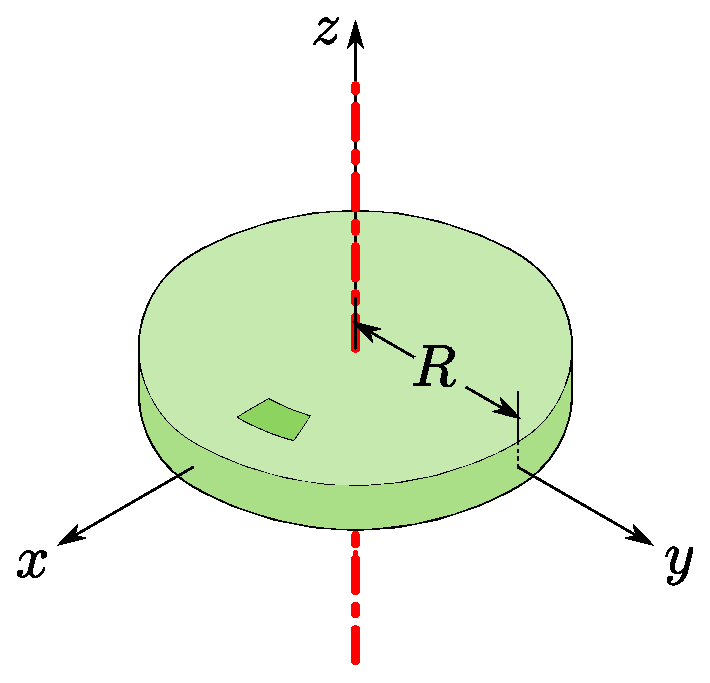
\includegraphics[scale=0.5]{resources/f13.eps}
\caption{Disco circular horizontal.}
\label{figura13}
\end{figure}

Considerando la \textbf{Ecuación (\ref{solidorigido})}:

\begin{equation*}
    I = \int_{M} r^2\, dm
\tag{4}
\end{equation*}

Asumiendo la distribución homogénea y superficial de la masa, y usando un
sistema de referencia polar:

\begin{equation*}
    \sigma = \frac{dm}{ds} = \frac{dm}{r\, d\theta\, dr}
\end{equation*}

Por tanto:

\begin{equation}
    dm = \sigma\, r\, d\theta\, dr
\label{dm8}
\end{equation}

Reemplazando (\ref{dm8}) en (\ref{solidorigido}):

\begin{equation*}
    I = \int_{M} r^2\, dm = \int_{0}^{R} \int_{0}^{2\pi} r^2\, \sigma\, r\, d\theta\, dr = \sigma \int_{0}^{R} \int_{0}^{2\pi} r^3\, d\theta\, dr = \sigma \int_{0}^{R} ( r^3\, \theta \Biggr|_{0}^{2\pi} )\, dr
\end{equation*}
\begin{equation*}
    I = \sigma \int_{0}^{R} 2\pi\, r^3\, dr = 2\pi\, \sigma \int_{0}^{R} r^3 dr = 2\pi\, \sigma\, \frac{r^4}{4} \Biggr|_{0}^{R} = 2\pi\, \sigma\, \frac{R^4}{4}
\end{equation*}
\begin{equation}
    I = \pi\, \sigma\, \frac{R^4}{2}
\label{resultado8}
\end{equation}

A partir de la ecuación (\ref{dm8}) sabemos que:

\begin{equation*}
    M = \sigma\, S = \sigma\, \pi\, R^2
\end{equation*}

Despejando $\sigma$ y reemplazando en la ecuación (\ref{resultado8}), obtenemos:

\begin{equation*}
    I = \pi\, \left( \frac{M}{\pi\, R^2} \right) \frac{R^4}{2}
\end{equation*}

Resultando finalmente:

\begin{equation}
    I = \frac{1}{2}\, M\, R^2
\end{equation}

\subsection{Disco circular vertical}
El procedimiento para hallar el momento de inercia de un disco circular delgado
(véase la \textbf{Figura \ref{figura14}}) con eje en el centro de masa y
paralelo a su radio ($R$), es el siguiente:

\begin{figure}
\centering
\includegraphics[scale=0.5]{resources/f14.eps}
\caption{Disco circular vertical.}
\label{figura14}
\end{figure}

Considerando la \textbf{Ecuación (\ref{solidorigido})}:

\begin{equation*}
    I = \int_{M} r^2\, dm
\tag{4}
\end{equation*}

Asumiendo la distribución homogénea y superficial de la masa, y usando un
sistema de referencia polar:

\begin{equation*}
    \sigma = \frac{dm}{ds} = \frac{dm}{r\, d\theta\, dr}
\end{equation*}

Por tanto:

\begin{equation}
    dm = \sigma\, r\, d\theta\, dr
\label{dm9}
\end{equation}

Considerando la relación trigonométrica entre la distancia perpendicular ($d$) y
el radio ($r$) del diferencial.

\begin{equation*}
    cos (\theta) = \frac{d}{r}
\end{equation*}

Por tanto:

\begin{equation}
    d = r\, cos(\theta)
\label{r9}
\end{equation}

Reemplazando (\ref{r9}) y (\ref{dm9}) en (\ref{solidorigido}): 

\begin{equation*}
    I = \int_{M} r^2\, dm = \int_{0}^{R} \int_{0}^{2\pi} r^2\, cos^2(\theta)\, \sigma\, r\, d\theta\, dr = \sigma \int_{0}^{R} r^3 \int_{0}^{2\pi} cos^2(\theta)\, d\theta\, dr
\end{equation*}
\begin{equation*}
    I = \sigma \int_{0}^{R} r^3 \left( \int_{0}^{2\pi} \frac{1}{2} + \frac{1}{2} cos(2\theta) \, d\theta \right) \, dr = \sigma \int_{0}^{R} r^3 \left( \frac{1}{2}\, \theta \Biggr|_{0}^{2\pi} + \frac{1}{4} sen(2\theta) \Biggr|_{0}^{2\pi} \right) \, dr 
\end{equation*}
\begin{equation*}
    I = \sigma \int_{0}^{R} r^3 \left( \pi + \frac{1}{4} sen(4\pi) - \frac{1}{4} sen(0) \right) \, dr = \sigma \int_{0}^{R} r^3 \pi dr = \pi\, \sigma \int_{0}^{R} r^3 dr = \pi\, \sigma \left( \frac{r^4}{4} \Biggr|_{0}^{R} \right)
\end{equation*}
\begin{equation}
    I = \pi\, \sigma\, \frac{R^4}{4}
\label{resultado9}
\end{equation}

A partir de la ecuación (\ref{dm9}) sabemos que:

\begin{equation*}
    M = \sigma\, \pi\, R^2
\end{equation*}

Despejando $\sigma$ y reemplazando en la ecuación (\ref{resultado9}):

\begin{equation*}
    I = \pi\, \left( \frac{M}{\pi\, R^2} \right) \frac{R^4}{4}
\end{equation*}

Resultando finalmente:

\begin{equation}
    I = \frac{1}{4}\, M\, R^2
\end{equation}

\subsection{Esfera hueca}
El procedimiento para hallar el momento de inercia de una esfera hueca
(véase la \textbf{Figura \ref{figura15}}) con eje en el centro de masa y con
radio ($R$), es el siguiente:

\begin{figure}
\centering
\includegraphics[scale=0.5]{resources/f15.eps}
\caption{Esfera hueca.}
\label{figura15}
\end{figure}

Asumiendo la distribución homogénea y longitudinal de la masa, y usando un
sistema de referencia esférico:

\begin{equation*}
    \sigma = \frac{dm}{ds}
\end{equation*}
\begin{equation*}
    ds = R\, d\phi\, R\, sen(\phi)\, d\theta
\end{equation*}
\begin{equation*}
    ds = R^2\, sen (\phi)\, d\phi\, d\theta
\end{equation*}

Por tanto:

\begin{equation}
    dm = \sigma\, ds = \sigma\, R^2\, sen (\phi)\, d\phi\, d\theta
\label{dm10}
\end{equation}

Considerando la relación trigonométrica entre $R$ y $r$:

\begin{equation}
    r = R\, sen (\phi)
\label{r10}
\end{equation}

Reemplazando (\ref{r10}) y (\ref{dm10}) en (\ref{solidorigido}): 

\begin{equation*}
    I = \int_{S} r^2\, \sigma\, ds = \int_{0}^{2\pi} \int_{0}^{\pi} R^2\, sen^2(\phi)\, \sigma\, R^2\, sen (\phi)\, d\phi\, d\theta = \int_{0}^{2\pi} \int_{0}^{\pi} \sigma R^4\, sen^3(\phi)\, d\phi\, d\theta
\end{equation*}
\begin{equation*}
    I = \sigma\, R^4\, \int_{0}^{2\pi} \int_{0}^{\pi}\, sen^3(\phi)\, d\phi\, d\theta = \sigma\, R^4\, \int_{0}^{2\pi} \int_{0}^{\pi} sen^2(\phi)\, sen(\phi)\, d\phi\, d\theta
\end{equation*}
\begin{equation*}
    I = \sigma\, R^4\, \int_{0}^{2\pi} \int_{0}^{\pi} (1 - cos^2(\phi))\, sen(\phi)\, d\phi\, d\theta
\end{equation*}
\begin{equation*}
    I = \sigma\, R^4\, \int_{0}^{2\pi} \left( \int_{0}^{\pi} sen(\phi)\, d\phi - \int_{0}^{\pi} cos^2(\phi)\, sen(\phi)\, d\phi\, \right) d\theta
\end{equation*}
\begin{equation*}
    I = \sigma\, R^4\, \int_{0}^{2\pi} \left( -cos(\phi)\Biggr|_{0}^{\pi} + \frac{cos^3(\phi)}{3}\Biggr|_{0}^{\pi} \right) d\theta
\end{equation*}
\begin{equation*}
    I = \sigma\, R^4\, \int_{0}^{2\pi} \left( -cos(\pi) + cos(0) + \frac{cos^3(\pi)}{3} - \frac{cos^3(0)}{3} \right) d\theta
\end{equation*}
\begin{equation*}
    I = \sigma\, R^4\, \int_{0}^{2\pi} \left( 1 + 1 - \frac{1}{3} - \frac{1}{3} \right) d\theta = \sigma\, R^4\, \int_{0}^{2\pi} \frac{4}{3} d\theta = \sigma\, \frac{4\, R^4}{3} \int_{0}^{2\pi} d\theta = \sigma\, \frac{4\, R^4}{3} ( \theta \Biggr|_{0}^{2\pi} )
\end{equation*}
\begin{equation}
    I = \sigma\, \frac{8\pi}{3} R^4
\label{resultado8}
\end{equation}

A partir de la ecuación (\ref{dm10}) sabemos que:

\begin{equation*}
    M = \sigma\, S = \sigma\, 4\pi\, R^2
\end{equation*}

Despejando $\sigma$ y reemplazando en la ecuación (\ref{resultado10}):

\begin{equation*}
    I = (\frac{M}{4\pi\, R^2})\, \frac{8\pi\, R^4}{3}
\end{equation*}

Resultando finalmente:

\begin{equation}
    I = \frac{2}{3}\, M\, R^2
\end{equation}

\subsection{Bloque rectangular}
El procedimiento para hallar el momento de inercia de un bloque rectangular
(véase la \textbf{Figura \ref{figura16}}) con eje en el centro de masa,
perpendicular a sus medidas ($a$, $b$) y paralelo a su medida ($c$),
es el siguiente:

\begin{figure}
\centering
\includegraphics[scale=0.5]{resources/f16.eps}
\caption{Bloque rectangular.}
\label{figura16}
\end{figure}

Considerando la \textbf{Ecuación (\ref{solidorigido})}:

\begin{equation*}
    I = \int_{M} r^2\, dm
\tag{4}
\end{equation*}

Asumiendo la distribución homogénea y volumétrica de la masa:

\begin{equation*}
    \rho = \frac{dm}{dv} = \frac{dm}{dx\, dy\, dz}
\end{equation*}

Por tanto:

\begin{equation}
    dm = \rho\, dx\, dy\, dz
\label{dm11}
\end{equation}

Considerando la relación trigonométrica entre $r$, $x$, $y$, $z$:

\begin{equation}
    r^2 = x^2 + y^2 + z^2
\label{r11}
\end{equation}

Reemplazando (\ref{r11}) y (\ref{dm11}) en (\ref{solidorigido}):

\begin{equation*}
    I = \int_{M} r^2\, dm = \int_{-c/2}^{c/2} \int_{-b/2}^{b/2} \int_{-a/2}^{a/2} (x^2 + y^2 + z^2)\, \rho\, dx\, dy\, dz
\end{equation*}
\begin{equation*}
    I = \rho\, \int_{-c/2}^{c/2} \int_{-b/2}^{b/2} \int_{-a/2}^{a/2} (x^2 + y^2 + z^2)\, dx \, dy
\end{equation*}
\begin{equation*}
    I = \rho\, \int_{-c/2}^{c/2} \int_{-b/2}^{b/2} \left( \int_{-a/2}^{a/2} x^2\, dx + \int_{-a/2}^{a/2} y^2\, dx + \int_{-a/2}^{a/2} z^2\, dx \right) \, dy\, dz
\end{equation*}
\begin{equation*}
    I = \rho\, \int_{-c/2}^{c/2} \int_{-b/2}^{b/2} \left( \frac{x^3}{3} \Biggr|_{-a/2}^{a/2} + y^2 x \Biggr|_{-a/2}^{a/2} + z^2 x \Biggr|_{-a/2}^{a/2} \right) \, dy\, dz
\end{equation*}
\begin{equation*}
    I = \rho\, \int_{-c/2}^{c/2} \int_{-b/2}^{b/2} \left( \frac{(\frac{a}{2})^3}{3} - \frac{(-\frac{a}{2})^3}{3} + y^2 \left( \frac{a}{2}\right) - y^2 \left( -\frac{a}{2}\right) + z^2 \left( \frac{a}{2}\right) - z^2 \left( -\frac{a}{2}\right) \right) \, dy\, dz
\end{equation*}
\begin{equation*}
    I = \rho\, \int_{_c/2}^{c/2} \int_{-b/2}^{b/2} \left( \frac{a^3}{12} + a\, y^2 + a\, z^2 \right) \, dy\, dz
\end{equation*}
\begin{equation*}
    I = \rho\, \int_{-c/2}^{c/2} \left( \int_{-b/2}^{b/2} \frac{a^3}{12}\, dy + \int_{-b/2}^{b/2} a\, y^2\, dy + \int_{-b/2}^{b/2} a\, z^2\, dy \right) dz
\end{equation*}
\begin{equation*}
    I = \rho\, \int_{-c/2}^{c/2} \left( \frac{a^3}{12}\, y \Biggr|_{-b/2}^{b/2} + a\, \frac{y^3}{3} \Biggr|_{-b/2}^{b/2} + a\, z^2 y \Biggr|_{-b/2}^{b/2} \right) dz
\end{equation*}
\begin{equation*}
    I = \rho\, \int_{-c/2}^{c/2} \left( \frac{a^3}{12}\, \left( \frac{b}{2} + \frac{b}{2} \right) + a\, \left( \frac{(\frac{b}{2})^3}{3} - \frac{(-\frac{b}{2})^3}{3} \right) + a\, z^2\, \left( \frac{b}{2} + \frac{b}{2} \right) \right) dz
\end{equation*}
\begin{equation*}
    I = \rho\, \int_{-c/2}^{c/2} \left( \frac{a^3\, b}{12} + \frac{a\, b^3}{12} + a\, b\, z^2 \right) dz = \rho\, \left( \frac{a^3\, b\, z}{12} \Biggr|_{-c/2}^{c/2} + \frac{a\, b^3\, z}{12} \Biggr|_{-c/2}^{c/2} + \frac{a\, b\, z^3}{3} \Biggr|_{-c/2}^{c/2} \right)
\end{equation*}
\begin{equation*}
    I = \rho\, \left( \frac{a^3\, b}{12} \left( \frac{c}{2} + \frac{c}{2} \right) + \frac{a\, b^3}{12} \left( \frac{c}{2} + \frac{c}{2} \right) + a\, b\, \left( \frac{(\frac{c}{2})^3}{3} - \frac{(-\frac{c}{2})^3}{3} \right) \right) = \rho\, \left( \frac{a^3\, b\, c}{12} + \frac{a\, b^3\, c}{12} + \frac{a\, b\, c^3}{12} \right)
\end{equation*}
\begin{equation}
    I = \frac{\rho}{12} (a^3\, b\, c + a\, b^3\, c + a\, b\, c^3)
\label{resultado11}
\end{equation}

A partir de la ecuación (\ref{dm11}) sabemos que:

\begin{equation*}
    M = \rho\, a\, b\, c
\end{equation*}

Despejando $\rho$ y reemplazando en la ecuación (\ref{resultado11}):

\begin{equation*}
    I = \frac{1}{12} \left( \frac{M}{a\, b\, c} \right) (a^3\, b\, c + a\, b^3\, c + a\, b\, c^3) = \frac{1}{12} M \left( \frac{a^3\, b\, c}{a\, b\, c} + \frac{a\, b^3\, c}{a\, b\, c} + \frac{a\, b\, c^3}{a\, b\, c} \right)
\end{equation*}

Resultando finalmente:

\begin{equation}
    I = \frac{1}{12}\, M (a^2 + b^2 + c^2)
\end{equation}

\subsection{Cilindro horizontal}
El procedimiento para hallar el momento de inercia de un cilindro solido
(véase la \textbf{Figura \ref{figura17}}) con eje en el centro de masa,
perpendicular a su radio ($R$) y paralelo a su altura ($h$), es el siguiente:

\begin{figure}
\centering
\includegraphics[scale=0.5]{resources/f17.eps}
\caption{Cilindro horizontal.}
\label{figura17}
\end{figure}

Considerando la \textbf{Ecuación (\ref{solidorigido})}:

\begin{equation*}
    I = \int_{M} r^2\, dm
\tag{4}
\end{equation*}

Asumiendo la distribución homogénea y volumétrica de la masa, y usando un
sistema de referencia cilíndrico:

\begin{equation*}
    \rho = \frac{dm}{dv} = \frac{dm}{r\, d\theta\, dr dz}
\end{equation*}

Por tanto:

\begin{equation}
    dm = \rho\, r\, d\theta\, dr dz
\label{dm12}
\end{equation}

Reemplazando (\ref{dm12}) en (\ref{solidorigido}):

\begin{equation*}
    I = \int_{M} r^2\, dm = \int_{-h/2}^{h/2} \int_{0}^{R} \int_{0}^{2\pi} r^2\, \rho\, r\, d\theta\, dr\, dz = \rho\, \int_{-h/2}^{h/2} \int_{0}^{R} \int_{0}^{2\pi} r^3\, d\theta\, dr\, dz
\end{equation*}
\begin{equation*}
    I = \rho\, \int_{-h/2}^{h/2} \int_{0}^{R} (r^3\, \theta \Biggr|_{0}^{2\pi})\, dr\, dz = \rho\, \int_{-h/2}^{h/2} \int_{0}^{R} 2\pi\, r^3\, dr\, dz = 2\pi\, \rho \int_{-h/2}^{h/2} \left(\frac{r^4}{4}\Biggr|_{0}^{R}\right) dz
\end{equation*}
\begin{equation*}
    I = 2\pi\, \rho \int_{-h/2}^{h/2} \frac{R^4}{4}\, dz = 2\pi\, \rho \left(\frac{R^4}{4}\, z\,\Biggr|_{-h/2}^{h/2}\right) = 2\pi\, \rho\, \left( \frac{R^4}{4} \left( \frac{h}{2} + \frac{h}{2} \right)  \right) = 2\pi\, \rho\, \frac{R^4}{4}\, h
\end{equation*}
\begin{equation}
    I = \frac{1}{2}\, \pi\, \rho\, R^4\, h
\label{resultado12}
\end{equation}

A partir de la ecuación (\ref{dm12}) sabemos que:

\begin{equation*}
    M = \rho\, V = \rho\, \pi\, R^2\, h
\end{equation*}

Despejando $\rho$ y reemplazando en la ecuación (\ref{resultado12}), obtenemos:

\begin{equation*}
    I = \frac{1}{2} \pi\, (\frac{M}{\pi\, R^2\, h})\, R^4\, h
\end{equation*}

Resultando finalmente:

\begin{equation}
    I = \frac{1}{2}\, M\, R^2
\end{equation}

\subsection{Cilindro vertical}
El procedimiento para hallar el momento de inercia de un disco circular delgado
(véase la \textbf{Figura \ref{figura18}}) con eje en el centro de masa,
paralelo a su radio ($R$) y perpendicular a su altura ($h$), es el siguiente:

\begin{figure}
\centering
\includegraphics[scale=0.5]{resources/f18.eps}
\caption{Cilindro vertical.}
\label{figura18}
\end{figure}

Considerando la \textbf{Ecuación (\ref{solidorigido})}:

\begin{equation*}
    I = \int_{M} r^2\, dm
\tag{4}
\end{equation*}

Asumiendo la distribución homogénea y volumétrica de la masa, y usando un
sistema de referencia cilíndrico:

\begin{equation*}
    \rho = \frac{dm}{dv} = \frac{dm}{r\, d\theta\, dr dz}
\end{equation*}

Por tanto:

\begin{equation}
    dm = \rho\, r\, d\theta\, dr\, dz
\label{dm13}
\end{equation}

Considerando la relación trigonométrica entre la distancia perpendicular ($d$) y
el radio ($r$) del diferencial.

\begin{equation*}
    cos (\theta) = \frac{d}{r}
\end{equation*}

Por tanto:

\begin{equation}
    d = r\, cos(\theta)
\label{r13}
\end{equation}

Considerando la relación trigonométrica entre la distancia perpendicular ($d$) y
el radio ($r$) del diferencial.

\begin{equation*}
    cos (\theta) = \frac{d}{r}
\end{equation*}

Por tanto:

\begin{equation}
    d = r\, cos(\theta)
\label{r9}
\end{equation}

Reemplazando (\ref{r9}) y (\ref{dm9}) en (\ref{solidorigido}): 

\begin{equation*}
    I = \int_{M} r^2\, dm = \int_{-h/2}^{h/2} \int_{0}^{R} \int_{0}^{2\pi} r^2\, cos^2(\theta)\, \rho\, r\, d\theta\, dr\, dz = \rho \int_{-h/2}^{h/2} \int_{0}^{R} r^3 \int_{0}^{2\pi} cos^2(\theta)\, d\theta\, dr\, dz
\end{equation*}
\begin{equation*}
    I = \rho \int_{-h/2}^{h/2} \int_{0}^{R} r^3 \left( \int_{0}^{2\pi} \frac{1}{2} + \frac{1}{2} cos(2\theta) \, d\theta \right) \, dr\, dz
\end{equation*}
\begin{equation*}
    I = \rho \int_{-h/2}^{h/2} \int_{0}^{R} r^3 \left( \frac{1}{2}\, \theta \Biggr|_{0}^{2\pi} + \frac{1}{4} sen(2\theta) \Biggr|_{0}^{2\pi} \right) \, dr\, dz
\end{equation*}
\begin{equation*}
    I = \rho \int_{-h/2}^{h/2} \int_{0}^{R} r^3 \left( \pi + \frac{1}{4} sen(4\pi) - \frac{1}{4} sen(0) \right) \, dr\, dz = \rho \int_{-h/2}^{h/2} \int_{0}^{R} r^3 \pi dr\, dz
\end{equation*}
\begin{equation*}
    I = \pi\, \rho \int_{-h/2}^{h/2} \int_{0}^{R} r^3 dr\, dz = \pi\, \rho \int_{-h/2}^{h/2} \left( \frac{r^4}{4} \Biggr|_{0}^{R} \right) dz = \pi\, \rho \int_{-h/2}^{h/2} \frac{R^4}{4}\, dz
\end{equation*}
\begin{equation*}
    I = \pi\, \rho\, \frac{R^4}{4} z \Biggr|_{-h/2}^{h/2} = \pi\, \rho \frac{R^4}{4}\, \left( \frac{h}{2} + \frac{h}{2} \right)
\end{equation*}
\begin{equation}
    I = \pi\, \rho\, \frac{R^4}{4}\, h
\label{resultado13}
\end{equation}

A partir de la ecuación (\ref{dm13}) sabemos que:

\begin{equation*}
    M = \rho\, V = \rho\, \pi\, R^2\, h
\end{equation*}

Despejando $\rho$ y reemplazando en la ecuación (\ref{resultado13}), obtenemos:

\begin{equation*}
    I = \pi\, (\frac{M}{\pi\, R^2\, h})\, \frac{R^4}{4}\, h
\end{equation*}

Resultando finalmente:

\begin{equation}
    I = \frac{1}{4}\, M\, R^2
\end{equation}

\subsection{Esfera solida}
El procedimiento para hallar el momento de inercia de una esfera solida
(véase la \textbf{Figura \ref{figura21}}) con eje en el centro de masa y con
radio ($R$), es el siguiente:

\begin{figure}
\centering
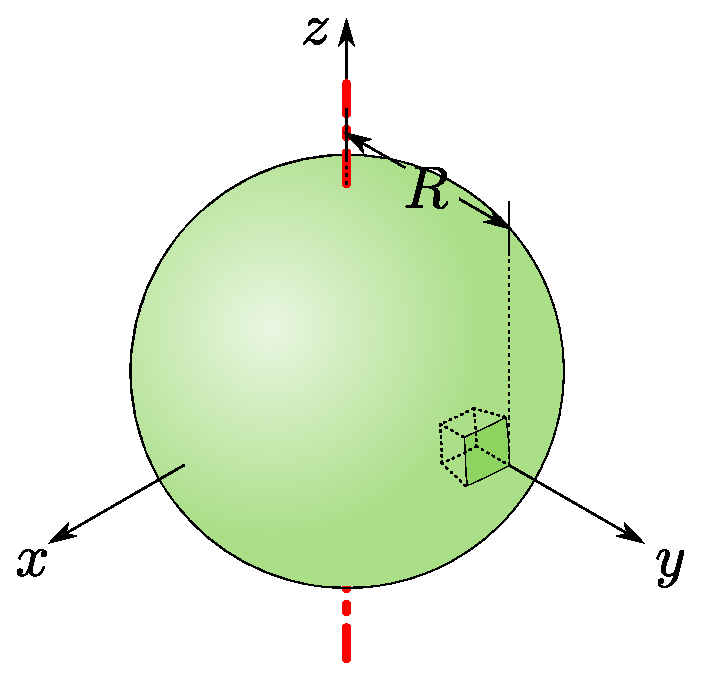
\includegraphics[scale=0.5]{resources/f21.eps}
\caption{Esfera solida.}
\label{figura21}
\end{figure}

Considerando la \textbf{Ecuación (\ref{solidorigido})}:

\begin{equation*}
    I = \int_{M} r^2\, dm
\tag{4}
\end{equation*}

Asumiendo la distribución homogénea y volumétrica de la masa, y usando un
sistema de referencia esférico:

\begin{equation*}
    \rho = \frac{dm}{dv}
\end{equation*}
\begin{equation*}
    dv = da\, a\, d\phi\, a\, sen (\phi)\, d\theta
\end{equation*}
\begin{equation*}
    dv = a^2\, sen (\phi)\, da\, d\phi\, d\theta
\end{equation*}

Por tanto:

\begin{equation}
    dm = \rho\, r\, d\theta\, dr\, dz
\label{dm16}
\end{equation}

Considerando la relación trigonométrica entre las variables $r$ y $a$:

\begin{equation}
    r = a\, sen (\phi)
\label{r16}
\end{equation}

Reemplazando (\ref{r16}) y (\ref{dm16}) en (\ref{solidorigido}): 

\begin{equation*}
    I = \int_{V} r^2\, \rho\, dv = \int_{0}^{2\pi} \int_{0}^{\pi} \int_{0}^{R} a^2\, sen^2(\phi)\, \rho\, a^2\, sen (\phi)\, da\, d\phi\, d\theta
\end{equation*}
\begin{equation*}
    I = \rho\, \int_{0}^{2\pi} \int_{0}^{\pi} \int_{0}^{R} a^4\, sen^3(\phi)\, da\, d\phi\, d\theta = \rho\, \int_{0}^{2\pi} \int_{0}^{\pi} \left(\frac{a^5}{5}\Biggr|_{0}^{R}\right)\, sen^3(\phi)\, d\phi\, d\theta
\end{equation*}
\begin{equation*}
    I = \rho\, \int_{0}^{2\pi} \int_{0}^{\pi} \frac{R^5}{5}\, sen^3(\phi)\, d\phi\, d\theta = \rho\, \frac{R^5}{5}\, \int_{0}^{2\pi} \int_{0}^{\pi} sen^3(\phi)\, d\phi\, d\theta
\end{equation*}
\begin{equation*}
    I = \rho\, \frac{R^5}{5}\, \int_{0}^{2\pi} \int_{0}^{\pi} sen^2(\phi)\, sen(\phi)\, d\phi\, d\theta = \rho\, \frac{R^5}{5}\, \int_{0}^{2\pi} \int_{0}^{\pi} (1 - cos^2(\phi))\, sen(\phi)\, d\phi\, d\theta
\end{equation*}
\begin{equation*}
    I = \rho\, \frac{R^5}{5}\, \int_{0}^{2\pi} \left( \int_{0}^{\pi} sen(\phi)\, d\phi - \int_{0}^{\pi} cos^2(\phi)\, sen(\phi)\, d\phi\, \right) d\theta
\end{equation*}
\begin{equation*}
    I = \rho\, \frac{R^5}{5}\, \int_{0}^{2\pi} \left( -cos(\phi)\Biggr|_{0}^{\pi} + \frac{cos^3(\phi)}{3}\Biggr|_{0}^{\pi} \right) d\theta
\end{equation*}
\begin{equation*}
    I = \rho\, \frac{R^5}{5}\, \int_{0}^{2\pi} \left( -cos(\pi) + cos(0) + \frac{cos^3(\pi)}{3} - \frac{cos^3(0)}{3} \right) d\theta
\end{equation*}
\begin{equation*}
    I = \rho\, \frac{R^5}{5}\, \int_{0}^{2\pi} \left( 1 + 1 - \frac{1}{3} - \frac{1}{3} \right) d\theta = \rho\, \frac{R^5}{5}\, \int_{0}^{2\pi} \frac{4}{3} d\theta = \rho\, \frac{4\, R^5}{15} \int_{0}^{2\pi} d\theta = \rho\, \frac{4\, R^5}{15} ( \theta \Biggr|_{0}^{2\pi} )
\end{equation*}
\begin{equation}
    I = \rho\, \frac{8\pi}{15}\, R^5
\label{resultado16}
\end{equation}

A partir de la ecuación (\ref{dm16}) sabemos que:

\begin{equation*}
    M = \rho\, V = \rho\, \frac{4\pi}{3} R^3
\end{equation*}

Despejando $\rho$ y reemplazando en la ecuación (\ref{resultado16}):

\begin{equation*}
    I = (\frac{3\, M}{4\pi\, R^3})\, \frac{8\pi\, R^5}{15}
\end{equation*}

Resultando finalmente:

\begin{equation}
    I = \frac{2}{5}\, M\, R^2
\end{equation}

\section{Piezas compuestas}
Los teoremas de los ejes paralelos hacen posible determinar los momentos de una
pieza compuesta en términos de un sistema coordenado específico, $xyz$, cuando
se conocen los momentos de cada parte del área compuesta en términos de un
sistema coordenado paralelo, con su origen en el centro de masa de la parte.
Los valores de los momentos de las partes en términos del sistema coordenado
$xyz$ pueden sumarse (o restarse en el caso de un recorte) para obtener los
valores del área compuesta \cite{Fowler}.

\begin{minipage}[c]{.4\linewidth}
\textbf{Ejemplo 4}:\\
Dada la pieza de la figura, determinar el momento de inercia en el eje
presentado.

Peso de la pieza: $1\, [kg]$.

\end{minipage}\hfill
\begin{minipage}{.5\linewidth}
\includegraphics[width=0.85\textwidth]{resources/f22.eps}
\end{minipage}
\\
\\

\begin{minipage}[b]{.9\linewidth}
\textbf{Solución}:\\
Para el calculo del momento de inercia de la pieza, esta será dividida en: un
rectángulo sin recorte, un semicírculo sin recorte, y un recorte circular.

Se usará la \textbf{ecuación (\ref{steiner})} para determinar el momento de
inercia en el eje para cada pieza. Y posteriormente se sumaran los resultados.
\\

\underline{Pieza 1 (Rectángulo)}:\\
Centro de masa:

\begin{equation*}
    CM = (60,0)
\end{equation*}

Momento de inercia:

\begin{equation*}
    I_{CM} = \frac{1}{12} M a^2 = \frac{1}{12} M (120)^2
\end{equation*}

Momento de inercia en el eje:

\begin{equation*}
    I_1 = I_{CM} + M d^2 = \frac{1}{12} M\, (120)^2 + M (60^2) = 4800 M
\end{equation*}

\underline{Pieza 2 (Semicírculo)}:\\
Centro de masa:

\begin{equation*}
    CM = \left( 120 + \frac{4R}{3\pi}, 0 \right) = \left( 120 + \frac{4 (40)}{3\pi}, 0 \right) = (136.98, 0)
\end{equation*}

Momento de inercia:

\begin{equation*}
    I_{CM} = \frac{2}{\pi} M R^2 \left( \frac{\pi}{8} - \frac{8}{9\pi} \right)
\end{equation*}

Momento de inercia en el eje:

\begin{equation*}
    I_2 = I_{CM} + M d^2 = \frac{2}{\pi} M (40)^2 \left( \frac{\pi}{8} - \frac{8}{9\pi} \right) + M (136.98)^2 = \num{1.8874e4} M
\end{equation*}

\underline{Pieza 3 (Circulo)}:\\
Centro de masa:

\begin{equation*}
    CM = (120, 0)
\end{equation*}

Momento de inercia:

\begin{equation*}
    I_{CM} = \frac{1}{4} M R^2
\end{equation*}

Momento de inercia en el eje:

\begin{equation*}
    I_3 = I_{CM} + M d^2 = \frac{1}{4} M R^2 + M (120)^2 = \frac{1}{4} M (20)^2 + M (120)^2 = 14500 M
\end{equation*}

El momento de inercia total es la suma de las partes:

\begin{equation*}
    I = I_1 + I_2 - I_3 = 9174.4 M = 9174.4 [kg\, mm^2]
\end{equation*}

\end{minipage}

\begin{thebibliography}{99}

\bibitem{FISIC.CH} Momento de Inercia \\
Extraído el 21 de Abril del 2021, de: \\
\url{https://www.fisic.ch/contenidos/din%C3%A1mica-rotacional/momento-de-inercia/}.
 
\bibitem{Sears} Sears y Zemansky (2013).\\
Física Universitaria. Volumen 1.\\
13va Edición.\\
Capitulo 9: Rotación de cuerpos rígidos.

\bibitem{WIKI1} Teorema del eje paralelo \\
Extraído el 25 de Abril del 2021, de: \\
\url{https://es.wikipedia.org/wiki/Teorema_del_eje_paralelo}.

\bibitem{Fowler} Berford, Anthony; Fowler, Wallacet (2008).\\
Mecánica para Ingeniería. Estática. \\
5ta Edición. \\
Capitulo 8: Momentos de inercia.

\end{thebibliography}

\end{document}

